
\section{Conceptos Previos}

\begin{frame}
    \frametitle{Optimización Global}
    \begin{block}{Definición Formal}
    El objetivo de la optimización global, considerando un problema de minimización, es encontrar un vector $X* \in \Omega$ tal que $f(X*) \leq f(X)$ para todo $X \in \Omega$.
    \end{block}
    \begin{block}{Espacio de Búsqueda}
    \textbf{El espacio de búsqueda} $\Omega$ está definido por un límite inferior ($a_{i}$) y superior ($b_{i}$) para cada una de las variables de decisión de la función, es decir: $\Omega = \prod^{D}_{i=1}[a_{i}, b{i}]$, siendo D el número de variables de decisión del problema a optimizar \citep{Segredo2017}
    \end{block}
\end{frame}

%++++++++++++++++++++++++++++++++++++++++++++++++++++++++++++++++++++++++++++++
\begin{frame} %TODO
\frametitle{Meta-heuristicas}
\begin{figure}
  \centering
	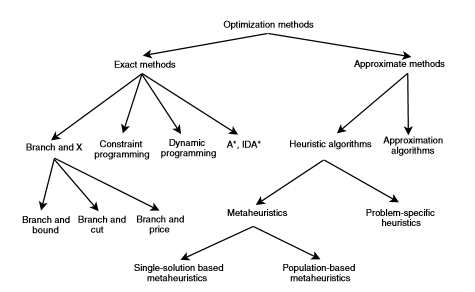
\includegraphics[scale=0.25]{img/meta}
\end{figure}
\end{frame}

%++++++++++++++++++++++++++++++++++++++++++++++++++++++++++++++++++++++++++++++
\begin{frame}
\frametitle{Meta-heuristicas}
\begin{block}{Categorías}
\begin{itemize}
    \item \textbf{Búsquedas Locales}: Greedy Randomized Adaptive Search Procedure (GRASP) \cite{GRASP}, Variable Neighborhood Search (VNS) \cite{vns}.
    \item \textbf{Heurísticas Voraces}: Simulated Annealing (SA) \cite{SA}.
    \item \textbf{Algoritmos Evolutivos}: Covariance Matrix Adaptation Evolutionary Strategy (CMA-ES) \cite{CMA}, Differential Evolution (DE) \cite{DE1, DE2, DE3}, Coevolutionary Algorithms (CEA) \cite{COE1, COE2, COE3}.
\end{itemize}
\end{block}
\end{frame}

%++++++++++++++++++++++++++++++++++++++++++++++++++++++++++++++++++++++++++++++
\begin{frame}
\frametitle{Meta-heuristicas}
\begin{block}{Criterios de Diseño}
\Fontvi
\begin{itemize}
	\item Intensificación.
	\item Diversificación.
	\item Representación.
    \begin{itemize}
    \item Permutaciones.
    \item Cadena binaria.
    \item Vector de valores naturales.
    \item \textbf{Vector de números reales}.
\end{itemize}
	\item Condición de parada.
    \begin{itemize}
    \item Iteraciones.
    \item Factor de error.
    \item \textbf{Evaluaciones}: $10^{6}$ evaluaciones establecidas por GenOpt.
\end{itemize}
	\end{itemize}
    \end{block}
\end{frame}

